
\section*{Problema P7.26}

\renewcommand*\thesection{7.26}
\numberwithin{equation}{section}

\begin{center}
    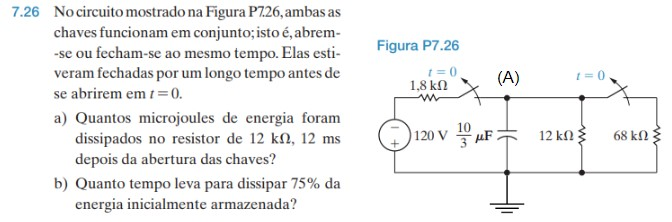
\includegraphics[scale=1.0]{P7.26.jpg}
\end{center}

\subsection*{(a)}

O primeiro passo é entender o que está acontencendo antes das chaves se abrirem, ou seja, quando $t<0$. Nesse caso, temos o capacitor atuando como um
circuito aberto. Assim, usando análise nodal no nó essencial (A),

\[ \frac{V_A - (-120)}{1.8\un{k}} + \frac{V_A}{12\un{k}} + \frac{V_A}{68\un{k}} = 0 \]

\[ V_A\left(\frac{1}{1.8\un{k}} + \frac{1}{12\un{k}} + \frac{1}{68\un{k}} \right) = - \frac{120}{1.8\un{k}} \]

\[ V_A = - \frac{\frac{120}{1.8\un{k}}}{\frac{1}{1.8\un{k}} + \frac{1}{12\un{k}} + \frac{1}{68\un{k}}}  \]

\[ V_A = v_c(0) = -102 \un{V} \]

Uma vez calculado a tensão inicial do capacitor, partimos para o $t>0$. Quando as chaves abrem, o capacitor descarrega no resistor $R_2 = 12 \un{k$\Omega$}$, resultando
na função já conhecida de descarga do capacitor 

\begin{equation}\label{eq:7.26.1}
    v(t) = v(0)e^{-\frac{t}{RC}} \un{V}
\end{equation}

Substituindo com os valores do exercício,   

\[ v(t) = -102e^{-25t} \un{V} \]

A potência dissipada no resistor $R_2$ é dada por 

\[ p(t) = \frac{[v(t)]^2}{R_2} = \frac{[-102e^{-25t}]^2}{12000} = 0.867e^{-50t} \un{W} \]

Integrando $p(t)$ no intervalo $0 \leq t \leq 12 \un{ms}$, temos a energia dissipada pelo resistor nesse período de tempo.

\[ E = \int_{0}^{12 \un{ms}} p(t) \,dt \]

\[ E = \int_{0}^{12 \un{ms}} 0.867e^{-50} \,dt \]

\[ E = 0.867 \frac{1}{-50} \left[e^{-50(12 \un{ms})} - e^{0}\right] \]

\[ \boxed{E = 7823.6 \un{$\mu$J}}  \]

\subsection*{(b)}

A energia em um capacitor é dada por  

\begin{equation}\label{eq:7.26.2}
    E(t) = \frac{1}{2}C[v(t)]^2
\end{equation}

Isolando $t$, 

\[ v(t) = \sqrt{\frac{2E(t)}{C}}  \]

Subsituindo \eqref{eq:7.26.1} na expressão acima, temos   

\[ e^{-\frac{t}{RC}} = \frac{1}{v_0} \sqrt{\frac{2E(t)}{C}}  \]

\[ -\frac{t}{RC} = \ln \left(\frac{1}{v_0} \sqrt{\frac{2E(t)}{C}}\right)   \]

\[ t = -RC\ln \left(\frac{1}{v_0} \sqrt{\frac{2E(t)}{C}}\right)   \]

Queremos que seja dissipado $75\%$ da energia inicial armazenada. Isso significa que precisamos de um instante $t$ tal que

\[ E(t) = 25\% E(0) = \frac{1}{4}E(0) = \frac{1}{4}\frac{1}{2}Cv_o^2 \]

Subsituindo esse $E(t)$ na expressão de $t$ acima,   

\[ t = -RC\ln \left(\frac{1}{v_0} \sqrt{\frac{2\frac{1}{4}\frac{1}{2}Cv_o^2}{C}}\right)  \]

\[ t = -RC\ln \left(\sqrt{\frac{1}{4}}\right)  \]

\[ t = -RC\ln \left(\frac{1}{2}\right)  \]

Subsituindo tudo,   

\[ \boxed{t = 27.725 \un{ms}}  \]

















